%----------------------------------------------------------------------------------------
%	PART II
%----------------------------------------------------------------------------------------

\part{The Nyxi}

%----------------------------------------------------------------------------------------
%	FIRST ENCOUNTER
%----------------------------------------------------------------------------------------

\chapterimage{placeholder.png} % Chapter heading image

\chapter{Physiology}

\section{Biology}

The Nyxi are

\section{Clades}

\subsection{Fadiglaux}

\begin{wrapfigure}{L}{0.4\textwidth}
	\centering
	
\includegraphics[width=0.38\textwidth]{clades/Fadiglaux.png}
\end{wrapfigure}

\lipsum[1]

\subsection{Baroquinfernum}

\begin{wrapfigure}{R}{0.4\textwidth}
	\centering
	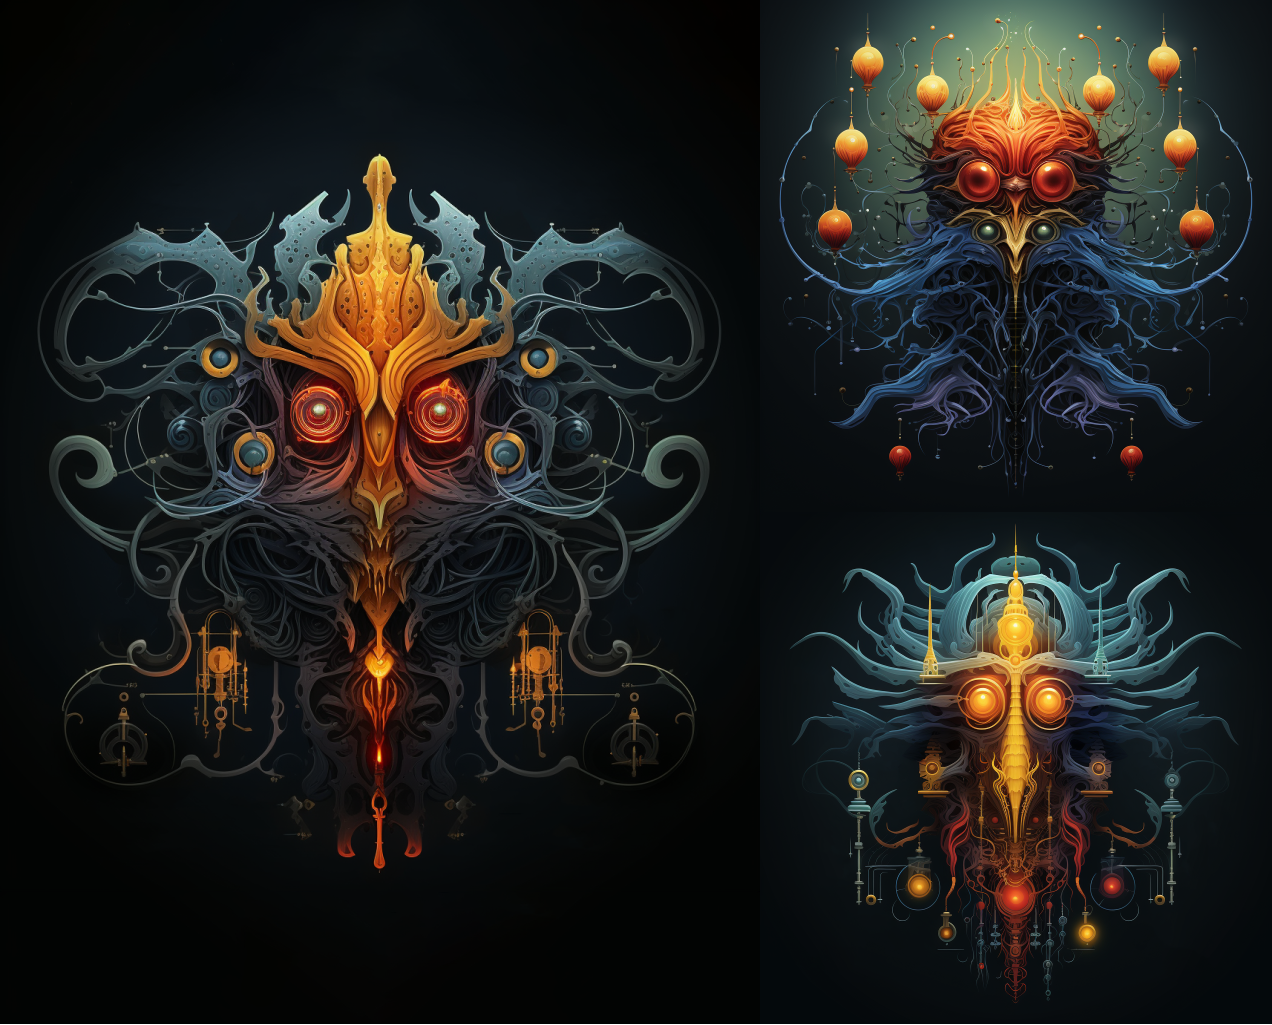
\includegraphics[width=0.38\textwidth]{clades/Baroquinfernum.png}
\end{wrapfigure}

\lipsum[2]

\subsection{Vanitavix}

\begin{wrapfigure}{L}{0.4\textwidth}
	\centering
	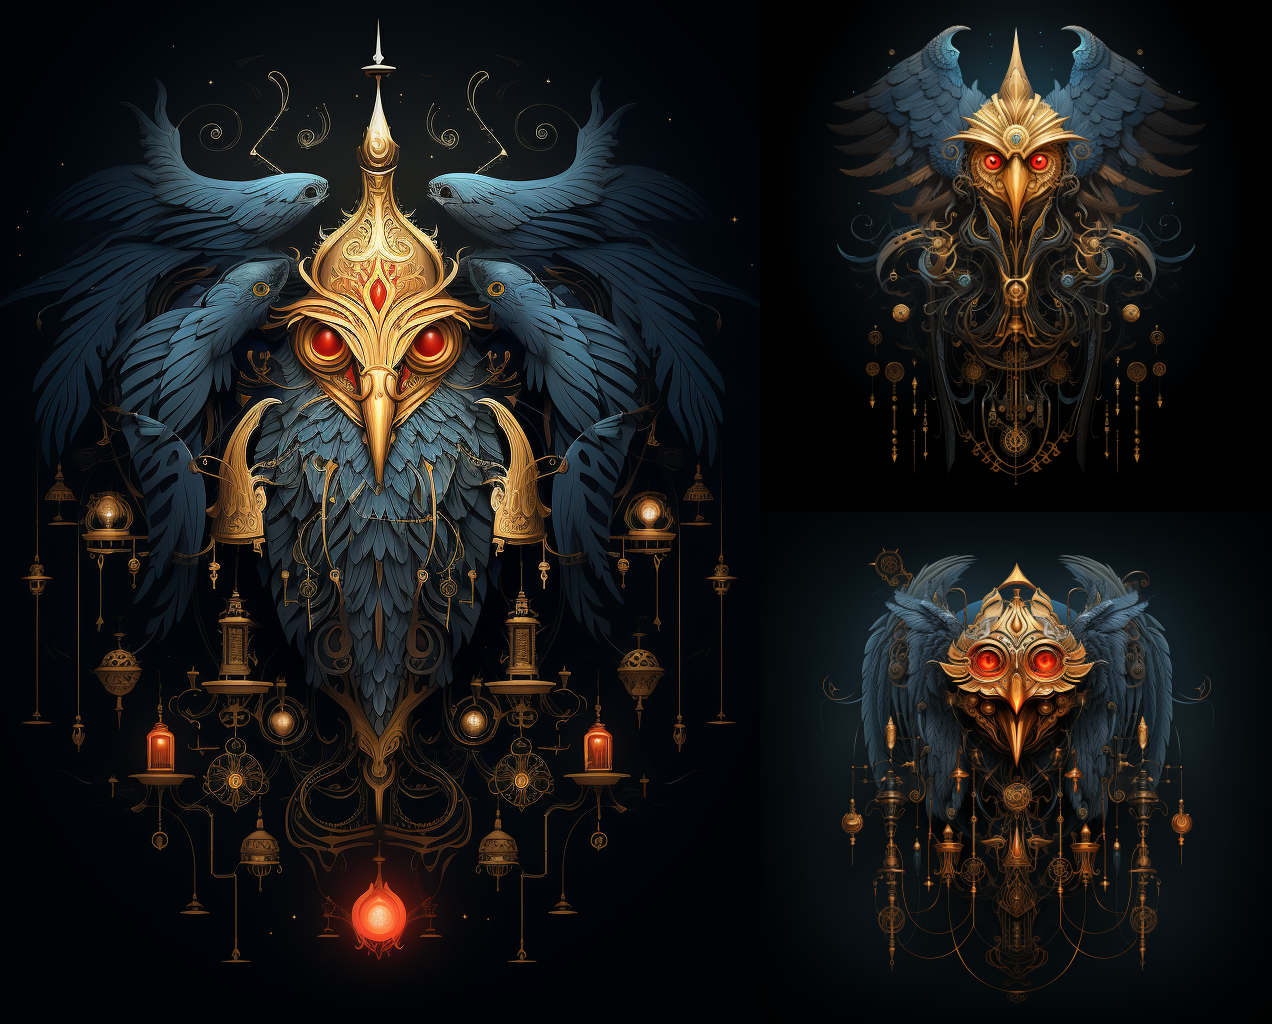
\includegraphics[width=0.38\textwidth]{clades/Vanitavix.png}
\end{wrapfigure}

\lipsum[3]

\subsection{Psychenyctua}

\begin{wrapfigure}{R}{0.4\textwidth}
	\centering
	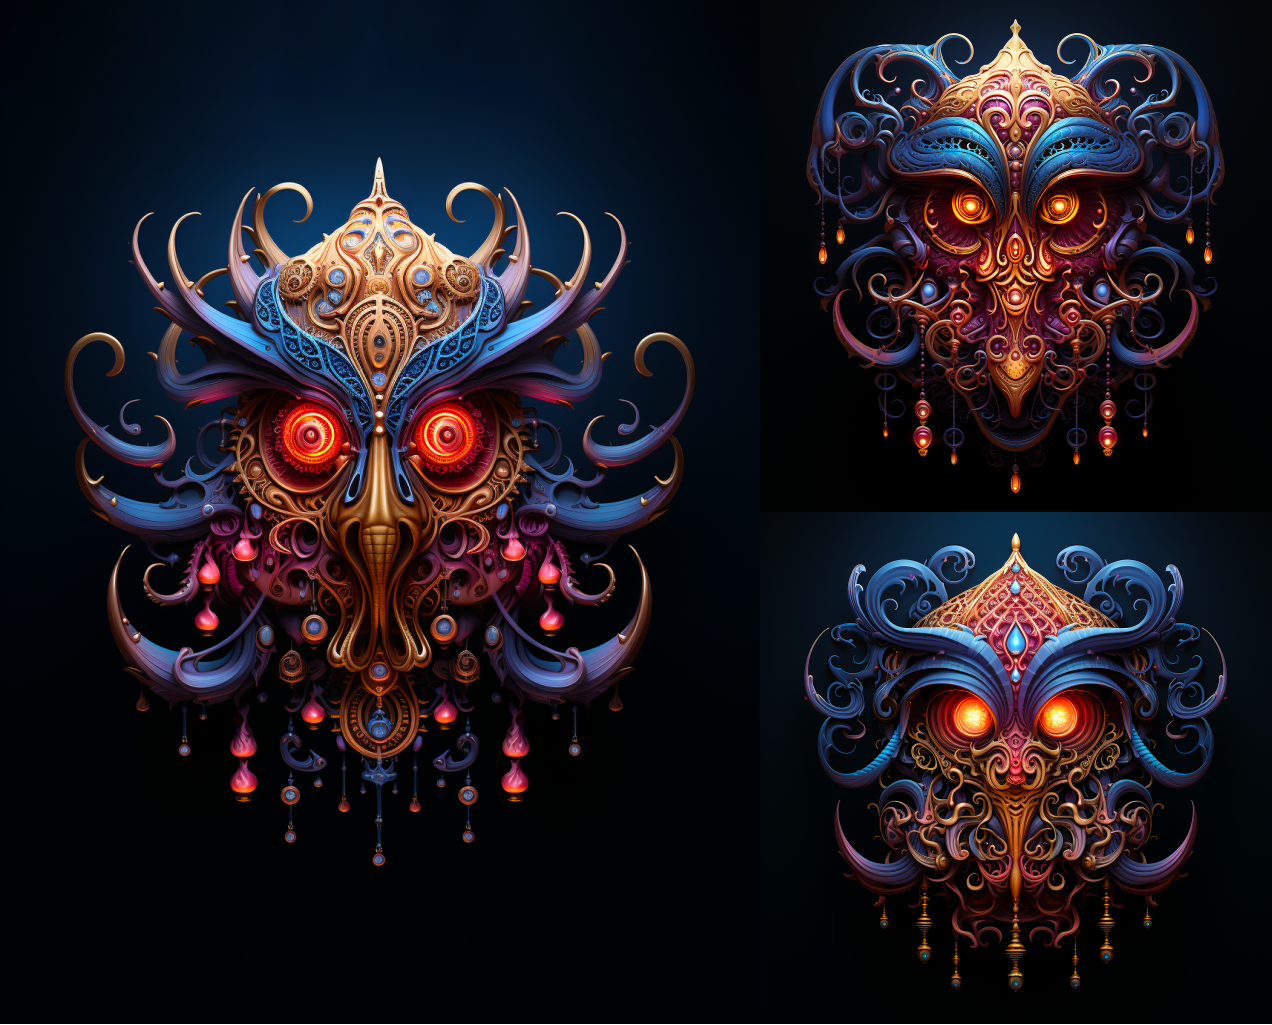
\includegraphics[width=0.38\textwidth]{clades/Psychenyctua.png}
\end{wrapfigure}

\lipsum[4]

\subsection{Sarkanagos}

\begin{wrapfigure}{L}{0.4\textwidth}
	\centering
	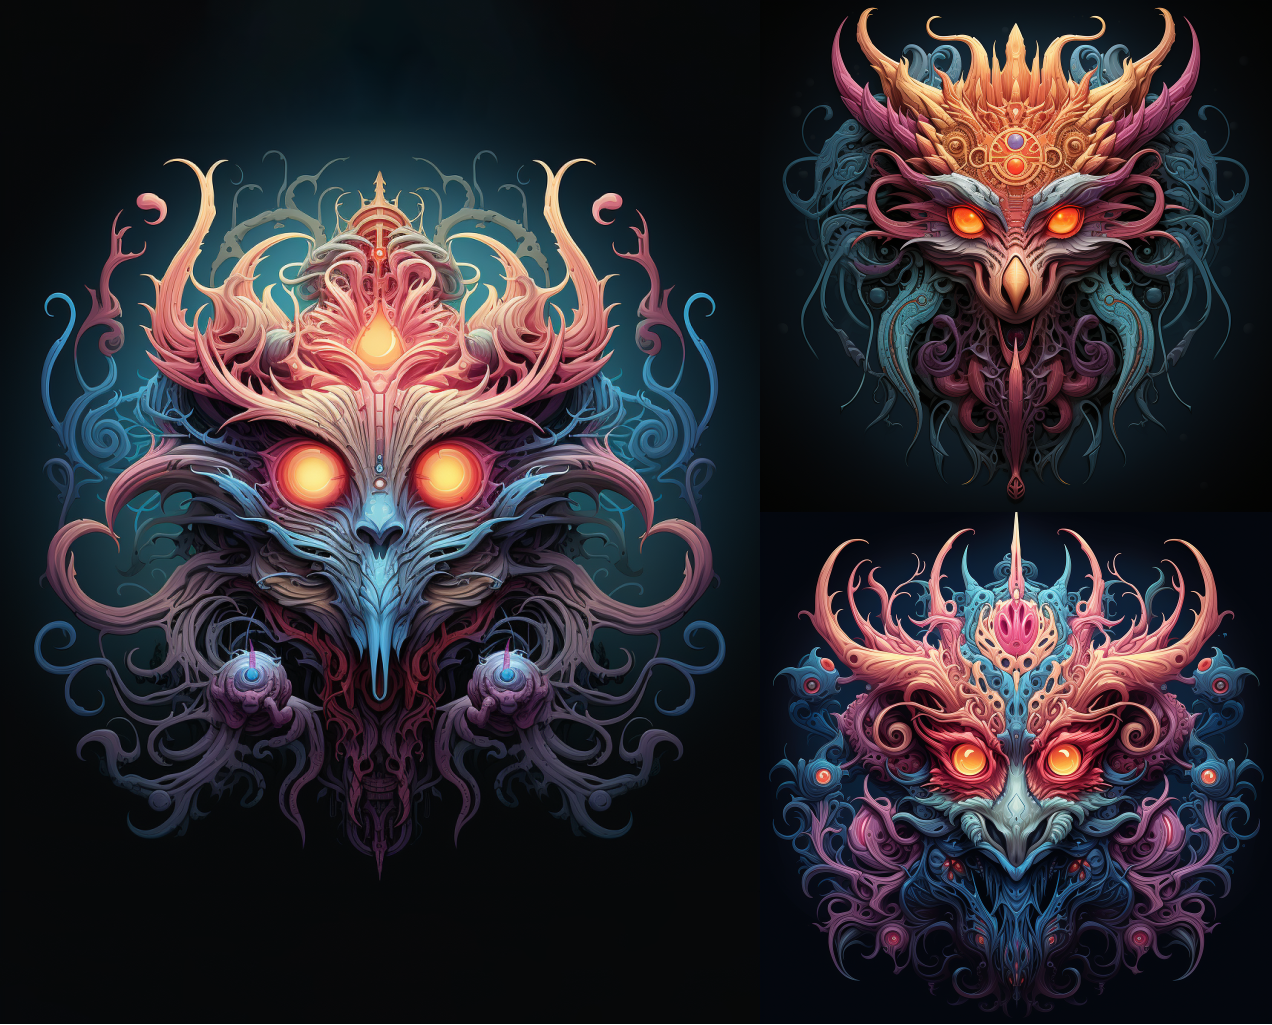
\includegraphics[width=0.38\textwidth]{clades/Sarkanagos.png}
\end{wrapfigure}

\lipsum[5]

\subsection{Ornatomedusa}

\begin{wrapfigure}{L}{0.4\textwidth}
	\centering
	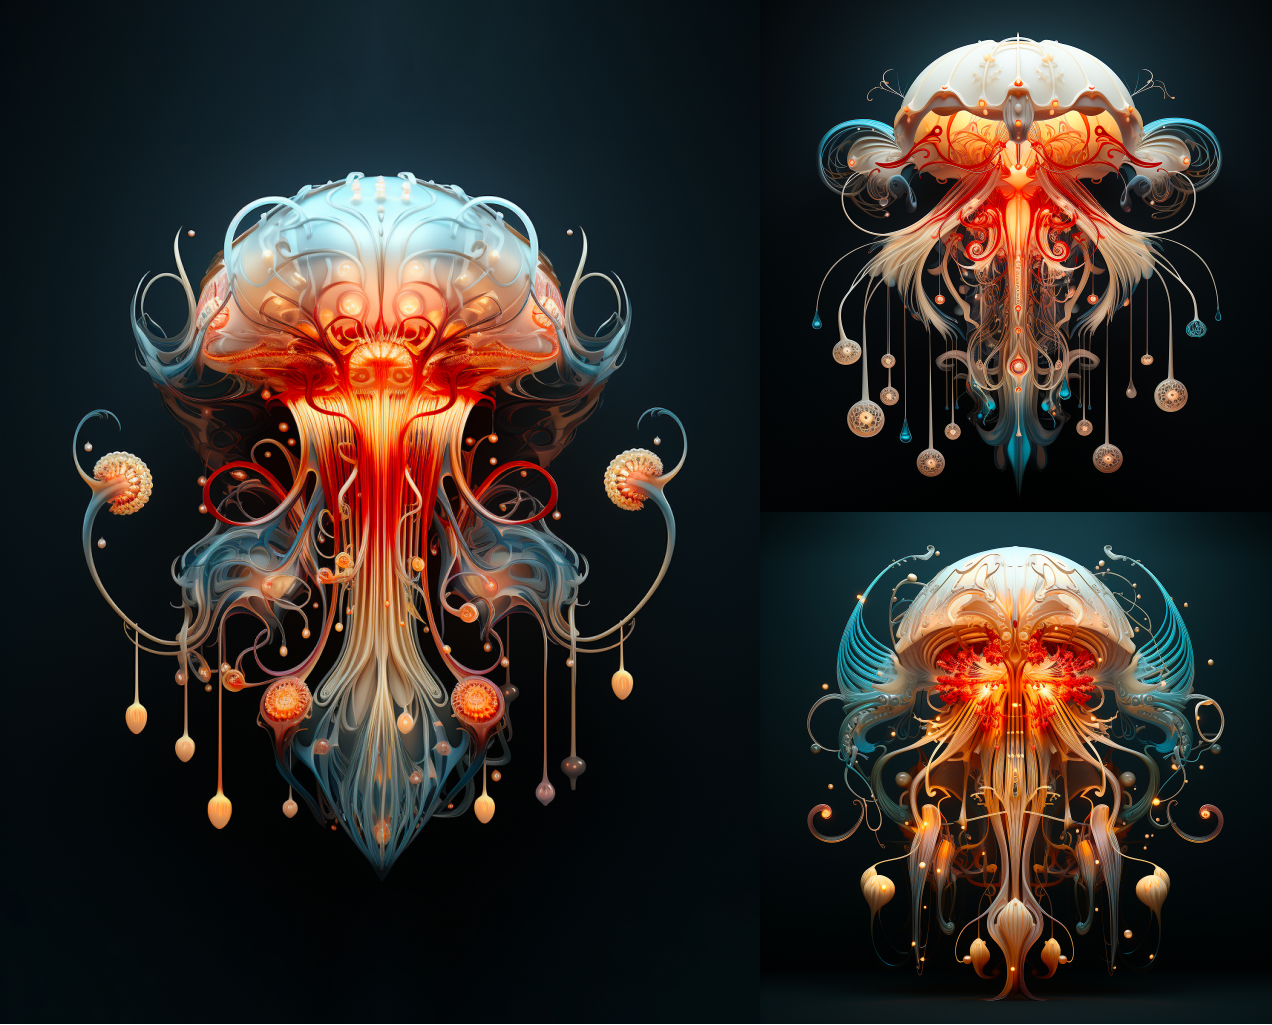
\includegraphics[width=0.38\textwidth]{clades/Ornatomedusa.png}
\end{wrapfigure}

\lipsum[6]

\subsection{Vakralakasha}

\begin{wrapfigure}{R}{0.4\textwidth}
	\centering
	
\includegraphics[width=0.38\textwidth]{clades/Vakralakasha.png}
\end{wrapfigure}

\lipsum[6]